\documentclass{article}

\providecommand{\finishEntry}[1][]{\end{document}} % please don't change this line
\providecommand{\startEntry}[1][]{\begin{document}} % please don't change this line


\usepackage[english]{babel}
\usepackage{amsmath}
\usepackage{amssymb}
\usepackage{amsthm}
\usepackage{physics} % for \abs{}
\usepackage{bm} % for \bm bold text

\usepackage{graphicx}

\graphicspath{ {./figures/} }

\DeclareMathOperator{\im}{Im} %Image

\newcommand{\nat}{\mathbb{N}}
\newcommand{\re}{\mathbb{R}}
\newcommand{\rat}{\mathbb{Q}} %rationals

\newcommand{\transpose}{\intercal}  %why on earth is this thing called an `intercal'?
\newcommand{\del}{\partial}

\newcommand{\dx}[1][x]{\text{d} #1 }  %usage $\dx$ -> dx, or $\dx[V]$ -> dV

\newcommand{\floor}[1]{\lfloor #1 \rfloor}
\newcommand{\ceil}[1]{\lceil #1 \rceil}

\theoremstyle{plain}
\newtheorem{thm}{Theorem}[section]
\newtheorem{lem}[thm]{Lemma}
\newtheorem{prop}[thm]{Proposition}
\newtheorem*{thmno}{Theorem}
\newtheorem*{lemno}{Lemma}
\newtheorem*{propno}{Proposition}


\theoremstyle{definition}
\newtheorem{defn}{Definition}[section]
\newtheorem*{defno}{Definition}

\theoremstyle{remark}
\newtheorem{rem}{Remark}
\newtheorem*{remno}{Remark}

% Please edit this file as you please so that it does what you want it to. ()
% This file is intended to contain all of the course independent macros and packages.
% If you need a specific package or command for just one course, that should be defined in that course's "preamble.tex"

% a friendly reminder to use \startEntry and \endEntry instead of \begin{document} and \end{document}
\startEntry{}
Today's lecture will be about frying.
\section{How to fry and egg}
There are lots of different ways to fry an egg, but they all do a similary thing: Heat the egg up so that it cooks in, but in a frying pan. I will now describe how to do this.
\begin{enumerate}
\item Put pan on heat
\item Add fat (oil, butter)
\item Let oil heat up a bit
\item Add egg
\item (Optional) Stir egg violently
\item When egg is no longer liquid, it is cookes
\item Remove egg
\item Take pan off heat
\end{enumerate}
I should probably mention that I have never cooked an egg before.
This is what it shoud look like:
\begin{figure}[h]
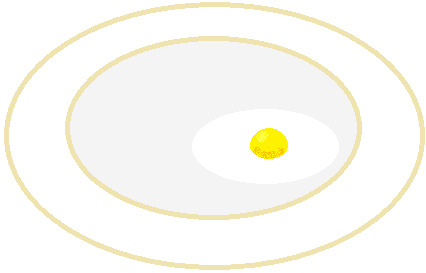
\includegraphics[width=8cm]{Egg_on_plate.png}
\end{figure}


Now isn't that a nice egg?
\finishEntry{}